% Build from this directory: latexmk -pdf -outdir=build background.tex
% Each chapter has deliberately placed page breaks and is at most five pages.
\documentclass[11pt,a4paper,oneside]{report}
\usepackage[T1]{fontenc}
\usepackage[utf8]{inputenc}
\usepackage{lmodern,microtype,textcomp}
\usepackage[margin=23mm,headheight=15pt]{geometry}
\usepackage{amsmath,amssymb,bm,mathtools}
\usepackage{booktabs,tabularx,array}
\usepackage{xcolor,tikz}
\usetikzlibrary{arrows.meta,positioning,calc}
\usepackage{listings,enumitem,titlesec,fancyhdr}
\usepackage[numbers,sort&compress]{natbib}
\usepackage{xurl}
\usepackage[colorlinks=true,linkcolor=blue!45!black,citecolor=blue!45!black,
  urlcolor=blue!50!black,pdftitle={Background for HPC Mini-Challenge 2}]{hyperref}
\definecolor{accent}{HTML}{165A72}
\definecolor{codebg}{HTML}{F3F6F8}
\definecolor{muted}{HTML}{52616B}
\titleformat{\chapter}[display]{\normalfont\bfseries\color{accent}}
  {\large Chapter \thechapter}{6pt}{\LARGE}
\titlespacing*{\chapter}{0pt}{0pt}{16pt}
\titleformat{\section}{\large\bfseries\color{accent}}{\thesection}{0.6em}{}
\titlespacing*{\section}{0pt}{11pt}{5pt}
\setlength{\parindent}{0pt}
\setlength{\parskip}{5pt plus 1pt}
\setlength{\emergencystretch}{3em}
\setlist{nosep,leftmargin=1.4em,topsep=4pt}
\setcounter{tocdepth}{0}
\pagestyle{fancy}
\fancyhf{}
\fancyhead[L]{\small\color{muted}\nouppercase{\leftmark}}
\fancyfoot[L]{\small\color{muted}HPC HS26 \enspace / \enspace Mini-Challenge 2}
\fancyfoot[R]{\thepage}
\renewcommand{\headrulewidth}{0.3pt}
\renewcommand{\chaptermark}[1]{\markboth{\thechapter\enspace #1}{}}
\fancypagestyle{plain}{\fancyhf{}\fancyfoot[L]{\small\color{muted}HPC HS26 / Mini-Challenge 2}\fancyfoot[R]{\thepage}\renewcommand{\headrulewidth}{0pt}}
\lstset{basicstyle=\ttfamily\fontsize{9}{10.7}\selectfont,
  backgroundcolor=\color{codebg},frame=single,rulecolor=\color{black!12},
  framerule=0.3pt,framesep=5pt,aboveskip=7pt,belowskip=7pt,
  keywordstyle=\color{accent}\bfseries,commentstyle=\color{muted},
  stringstyle=\color{green!35!black},showstringspaces=false,upquote=true,
  columns=fullflexible,keepspaces=true,breaklines=true,tabsize=4}
\lstdefinestyle{python}{language=Python}
\lstdefinestyle{shell}{language=bash}
\newcommand{\R}{\mathbb{R}}
\newcommand{\softmax}{\operatorname{softmax}}
\newcommand{\LN}{\operatorname{LN}}
\newcommand{\MHA}{\operatorname{MHA}}
\newcommand{\FFN}{\operatorname{FFN}}
\newcommand{\diag}{\operatorname{diag}}
\newcommand{\code}[1]{\texttt{\detokenize{#1}}}
\newcommand{\purpose}[1]{\textbf{Connection to the challenge.} #1\par}
\newcommand{\checkpoint}[1]{\medskip\textbf{Check your understanding.} #1\par}
\newcolumntype{Y}{>{\raggedright\arraybackslash}X}
% Keep the original five-page limit enforceable when editing definitions.
\newcounter{chapterstartpage}
\newcommand{\checkchapterlength}{%
  \ifnum\numexpr\value{page}-\value{chapterstartpage}\relax>4
    \PackageError{background}{Chapter \thechapter\space exceeds five pages}%
      {Shorten the chapter or adjust its page breaks.}%
  \fi}
\begin{document}
\hypersetup{pageanchor=false}
\begin{titlepage}
\vspace*{22mm}
{\large\color{accent}HIGH PERFORMANCE COMPUTING (HPC) \quad HS26\par}
\vspace{12mm}
{\Huge\bfseries Background for\\[5pt]Mini-Challenge 2\par}
\vspace{9mm}
{\Large Vision transformers, cluster execution,\\and performance measurement\par}
\vspace{16mm}
This report supplies the background for autumn semester 2026 (HS26) and the ten experiments in the
repository's \code{README.md}. It develops a small image classifier from
tensor operations, then explains how to run and measure it. Examples are
teaching building blocks, not measured results or a completed submission.

\vspace{6mm}
\textbf{Prerequisites:} basic Python, matrix multiplication, partial derivatives,
and familiarity with a command-line shell. Read Chapters 1--3 before building
the baseline; use Chapters 4--5 when running and interpreting experiments.


\vfill
{\large 4 November 2026\par}
\small References link to primary papers and official documentation. Online
application programming interfaces (APIs)
and cluster policies can change; record the versions and settings actually used.
\end{titlepage}
\pagenumbering{roman}
\hypersetup{pageanchor=true}
\tableofcontents
\vspace{10mm}
The examples use a central processing unit (CPU) locally and a graphics
processing unit (GPU) on the cluster. NVIDIA's Compute Unified Device
Architecture (CUDA) is the GPU computing platform used here. Scaled
Dot-Product Attention (SDPA) is the attention operation developed in Chapter 2.

\textbf{How the chapters support the experiments}
\begin{center}
\begin{tabularx}{\textwidth}{@{}lY@{}}
\toprule
Chapter & Experiments and questions supported\\\midrule
1 & Dataset, optimization, validation, reproducibility, full training (1, 8--10).\\
2 & Manual attention, gradients, vectorization, SDPA comparisons (1, 5--7).\\
3 & Architecture, tensor shapes, correctness, compilation (1, 2, 6, 10).\\
4 & CPU/GPU allocations, job scripts, output, resource accounting (3, 8, 10).\\
5 & Graphs, timing, memory, profiler overhead, loading, synchronization (2--10).\\
\bottomrule
\end{tabularx}
\end{center}
The optional mixed-precision and multi-GPU goals extend this foundation; they
do not change the required 32-bit floating-point (FP32), single-GPU comparisons. Each numbered chapter
is limited to five pages. Front matter and references are separate.

\textbf{Notation.} $\R$ denotes the real numbers; $\R^{m\times n}$ is the
space of matrices with $m$ rows and $n$ columns. A superscript
$\mathsf T$ denotes transpose, and a colon in an index selects an entire
axis. Token vectors are rows. $\exp$ and $\log$ are the natural exponential
and logarithm. Symbols reused in another section are defined there again.
\clearpage
\pagenumbering{arabic}

\chapter{PyTorch Introduction}\label{ch:pytorch}
\setcounter{chapterstartpage}{\value{page}}
\purpose{Build a trainable CPU baseline, move it to the allocated GPU, and
keep the data, model, and optimization settings reproducible.}

\section{Tensors describe both data and computation}
A tensor is an array with a shape, a data type, a device, and a memory layout.
An image batch has shape $(B,C,H,W)$: $B$ is the batch size, $C$ the number
of channels, and $H,W$ the image height and width in pixels. Tokens have
shape $(B,N,D)$, where $N$ is the number of tokens per image and $D$ the
number of features per token (the embedding width). Labels have shape $(B,)$ with integer values in
$\{0,\ldots,364\}$. A dimension's meaning matters as much as its length.
PyTorch's introductory tutorials provide the basic API vocabulary~\cite{pytorchbasics}.

\begin{lstlisting}[style=python]
import torch
from torch import nn
import torch.nn.functional as F

torch.manual_seed(17)
torch.set_float32_matmul_precision("highest")
device = torch.device("cpu")  # use "cuda:0" inside a GPU allocation
x = torch.randn(8, 64, 128, device=device, dtype=torch.float32)
projection = nn.Linear(128, 128).to(device=device, dtype=torch.float32)
z = projection(x)             # (8, 64, 128)
assert z.device == x.device
\end{lstlisting}

\begin{tabularx}{\textwidth}{@{}lY@{}}
\toprule
Operation & Meaning and common mistake\\\midrule
\code{a * b} & Elementwise multiplication with broadcasting; not matrix multiplication.\\
\code{a @ b} & Matrix multiplication on the last two dimensions; preceding dimensions broadcast.\\
\code{x.transpose(-2,-1)} & Exchange two axes; generally changes strides without copying data.\\
\code{x.reshape(...)} & Change shape; may copy if the current strides cannot represent it.\\
\code{x.to(device)} & Return a tensor on the chosen device; use the returned value.\\
\bottomrule
\end{tabularx}

Broadcasting aligns dimensions from the right; dimensions must match or one
must equal one. Thus a bias of shape $(D,)$ is shared by all $BN$ tokens.
Check shapes explicitly: accidental broadcasting can give plausible values
while computing the wrong function. A transposed tensor can be non-contiguous;
calling \code{view} on it may fail, while a later copy can affect performance.

\section{Modules own parameters}
An \code{nn.Module} defines \code{forward} and registers trainable
parameters and child modules. Use \code{nn.Parameter} for a learned tensor.
The \code{model.parameters()} iterator exposes parameters to an optimizer;
\code{model.to(device)} moves registered state.
Use \code{nn.ModuleList} for a collection of blocks so that their parameters
are registered. A linear layer applies $z=xW^{\mathsf T}+b$: input row $x$
has $D_{\rm in}$ features, output row $z$ has $D_{\rm out}$ features,
$W\in\R^{D_{\rm out}\times D_{\rm in}}$ is the stored weight matrix,
and $b\in\R^{1\times D_{\rm out}}$ is the broadcast bias row.
Below, mathematical weights multiply on the right and are stored transposed
by PyTorch. In the code, \code{x} and \code{z} hold whole batches of rows;
\code{nn} names the neural-network module namespace and \code{F} its functional interface.

\newpage
\section{Automatic differentiation and the objective}
Let $\theta\in\R^{P_\theta}$ collect the classifier's $P_\theta$ trainable
parameters. For sample index $b=1,\ldots,B$, $x_b$ is an input image,
$f_\theta$ the classifier, $s_b=f_\theta(x_b)\in\R^{365}$ its logit vector,
and $y_b\in\{0,\ldots,364\}$ the target class. The scalar batch loss
$\mathcal L(\theta)$ is mean cross-entropy, with class index $c$:
\begin{equation}
 \mathcal L(\theta)=\frac1B\sum_{b=1}^{B}
 \left[-s_{b,y_b}+\log\!\left(\sum_{c=0}^{364}e^{s_{b,c}}\right)\right].
\end{equation}
Pass logits directly to \code{F.cross_entropy}; applying softmax first changes
the intended input. PyTorch uses a numerically stable implementation. An epoch
is a pass through the training set; a step is one batch update. Their lengths
change differently when batch size changes.

Autograd applies the chain rule in reverse. Let $u=g(\theta)\in\R^m$ be an
intermediate activation vector with $m$ entries, where $g$ maps parameters
to activations and $h$ maps activations to the scalar loss $\mathcal L=h(u)$.
Then $\nabla_\theta\mathcal L=J_g(\theta)^{\mathsf T}\nabla_u h$.
Here $J_g\in\R^{m\times P_\theta}$ is the Jacobian of $g$ and
$\nabla$ denotes a gradient; the full Jacobian need not be formed.
Model parameters are usually leaf tensors with
\code{requires_grad=True}. Ordinary image inputs need not require gradients.
Calling \code{backward()} accumulates into parameter \code{.grad} fields;
gradients must therefore be cleared for independent updates~\cite{autograd}.

\begin{lstlisting}[style=python]
def train_step(model, optimizer, images, labels):
    optimizer.zero_grad(set_to_none=True)
    logits = model(images)
    loss = F.cross_entropy(logits, labels)
    loss.backward()
    optimizer.step()
    return loss.detach()  # metric without retaining the graph

# Construct the optimizer after placing the model on its device.
# model = TinyViT().to(device=device, dtype=torch.float32)  # Chapter 3
# optimizer = torch.optim.AdamW(model.parameters(), lr=3e-4)
# model.train()
# loss_on_device = train_step(model, optimizer, images, labels)
\end{lstlisting}

The challenge's training step comprises forward, loss, backward, and optimizer
work; the example also clears gradients. \code{detach()} removes a tensor from
the differentiation graph, but does not transfer it to the CPU. Saving the
original loss tensor in a list can retain graph state and grow memory use.
Use fresh forwards for subsequent steps; ordinary training does not need
\code{retain_graph=True}.

\section{What an optimizer changes}
Stochastic gradient descent uses
$\theta_{t+1}=\theta_t-\eta\nabla_\theta\mathcal L_t$, where $t$ is the
update index, $\theta_t$ the current parameters, $\mathcal L_t$ the current
batch loss, and $\eta>0$ the learning rate. AdamW is adaptive moment estimation
(Adam) with decoupled weight decay. It maintains first and second moment estimates for
each parameter and applies decoupled weight decay. Its state consumes memory
and may be initialized lazily at the first update. Fix optimizer type,
hyperparameters, and state across implementation comparisons~\cite{optimizing}.

\code{model.train()} and \code{model.eval()} set the model's training and
evaluation modes; neither switches autograd off. Validation uses evaluation mode and a
\code{torch.no_grad()} or \code{torch.inference_mode()} context. Return to
training mode afterwards.

\checkpoint{Why does a forward-only timing omit much of a training step?
Why do two consecutive calls to \code{backward()} on separate forwards still
require clearing gradients?}

\newpage
\section{Datasets, transformations, and loaders}
A map-style dataset supplies a sample by index; a \code{DataLoader} selects
indices, loads samples, and collates them into batches. The challenge uses
Places365-Standard, with separate training and validation splits. The prepared
shared copy must include the image layout and metadata expected by torchvision;
\code{small=True} selects the $256\times256$ source images~\cite{places365}.

The following deterministic transformation resizes red, green, and blue (RGB)
images to $128\times128$ for
a compact example model. Its normalization constants are an explicit example
choice, not statistics estimated from this dataset. Record and freeze the
transformation. Never estimate preprocessing statistics using validation data.

\begin{lstlisting}[style=python]
import os
from torchvision import datasets, transforms
from torch.utils.data import DataLoader, Subset

transform = transforms.Compose([
    transforms.Resize((128, 128)),
    transforms.ToTensor(),             # RGB uint8 -> float in [0, 1]
    transforms.Normalize((0.485, 0.456, 0.406),
                         (0.229, 0.224, 0.225)),
])
root = os.environ["PLACES365_ROOT"]     # shared, prepared copy
train_data = datasets.Places365(root, split="train-standard",
    small=True, download=False, transform=transform)
val_data = datasets.Places365(root, split="val",
    small=True, download=False, transform=transform)

subset_rng = torch.Generator().manual_seed(17)
indices = torch.randperm(len(train_data), generator=subset_rng)[:512]
dev_data = Subset(train_data, indices.tolist())
torch.save(indices, "development_indices.pt")

workers = 0  # change only within the available CPU allocation
worker_options = ({"prefetch_factor": 2, "persistent_workers": True}
                  if workers > 0 else {})
train_loader = DataLoader(dev_data, batch_size=32, shuffle=True,
    num_workers=workers, pin_memory=(device.type == "cuda"),
    generator=torch.Generator().manual_seed(29), **worker_options)
val_loader = DataLoader(val_data, batch_size=32, shuffle=False,
    num_workers=workers, pin_memory=(device.type == "cuda"),
    **worker_options)
\end{lstlisting}

For the final experiment use \code{train_data}, not \code{dev_data}, and cover
at least one complete training epoch. Keep a fixed validation subset for quick
development if needed, but identify it explicitly. A tiny-subset overfitting
check measures the ability to optimize; it is not held-out accuracy.

With zero workers, fetching occurs in the main process; positive worker counts
create subprocesses. Let $w$ be the number of workers and $p$ the prefetch
factor (batches prepared in advance per worker). For $w>0$, up to roughly
$wp$ batches can be queued, in addition to batches being processed. More
workers therefore change host memory demand as well as concurrency. Pinning
uses page-locked host memory. It can assist transfers but does not by itself
establish overlap~\cite{dataloader}.

Put script execution and loader creation under
\code{if __name__ == "__main__":} when using multiprocessing. Seed Python,
NumPy, and worker-side random transforms if used; the deterministic transform
above avoids that additional source of variation.

\newpage
\section{Training, validation, and recoverable runs}
Move both images and integer labels to the device before calling
\code{train_step}. Keep metrics on the device until a logging boundary.
For batch index $k$, let $B_k$ be its image count and $\mathcal L_k$ its mean
loss. Accumulate $B_k\mathcal L_k$ and divide by the total image count;
averaging batch means gives a smaller final batch too much weight.

\begin{lstlisting}[style=python]
@torch.no_grad()
def validate(model, loader, device):
    model.eval()
    totals = torch.zeros(2, device=device)  # loss sum, correct count
    count = 0
    for images, labels in loader:
        images = images.to(device, non_blocking=True)
        labels = labels.to(device, non_blocking=True)
        logits = model(images)
        totals[0] += F.cross_entropy(logits, labels, reduction="sum")
        totals[1] += (logits.argmax(dim=1) == labels).sum()
        count += labels.numel()
    values = (totals / count).cpu().tolist()  # one final host read
    return {"loss": values[0], "accuracy": values[1]}
\end{lstlisting}

Call \code{model.train()} at the start of each training epoch. Validate on
held-out images and never call the optimizer during validation. Record loss
and accuracy against examples processed and against elapsed time, since the
two plots answer different questions about learning and execution speed.

\begin{lstlisting}[style=python]
# Save after completing an epoch; config contains model/data/settings.
torch.save({"model": model.state_dict(),
            "optimizer": optimizer.state_dict(),
            "epoch": epoch, "config": config,
            "torch_rng": torch.get_rng_state()}, "checkpoint.pt")
\end{lstlisting}

For an exact resume also save CUDA, Python, NumPy, sampler/loader-generator,
and scheduler states as applicable. Resuming halfway through an epoch requires
tracking data position and worker randomness. A checkpoint of weights alone
does not restore optimizer moments or the subsequent sample order. Use a
separate initial checkpoint for controlled eager/compiled/SDPA comparisons.

\section{Reproducibility is an experimental design choice}
Record the seed, saved subset indices, transformations, package versions,
CPU/GPU model, thread count, model configuration, optimizer, data order, and
precision. A seed does not guarantee bitwise agreement across hardware or
algorithms. Small FP32 differences are expected; document tolerances and
compare learning over a common budget. For CPU experiments set
\code{torch.set_num_threads(n)} before computation; $n$ is the number of
CPU threads used for numerical operations.

The required precision setting controls float32 matrix multiplication, not
every backend independently. If adding convolutions, disable their TensorFloat-32 (TF32) mode
using the controls supported by the installed PyTorch version. Do not enable
autocast in required experiments. The linear patch embedding in Chapter 3
avoids a convolution-specific setting.

Use Weights \& Biases (W\&B) to associate configuration, Slurm job identifier (ID), metrics, and system samples
with one run. For disconnected compute nodes use offline logging and synchronize
later from a machine with access. Save raw measurements locally as comma-separated
values (CSV) or JavaScript Object Notation (JSON)
so the report notebook can regenerate plots without rerunning training.
Network logging and scalar extraction belong outside short benchmark windows.

\checkpoint{Verify shapes, finite loss/gradients, parameter updates, and
tiny-subset learning before profiling. Why do these checks not prove generalization?}

\checkchapterlength
\chapter{Scaled Dot-Product Attention}\label{ch:attention}
\setcounter{chapterstartpage}{\value{page}}
\purpose{Implement the manual baseline, explain every axis, and check that
alternative attention implementations compute the same function and gradients.}

\section{One head: definitions before implementation}
For one sample and one head, $Q\in\R^{N_q\times d_k}$ is the query matrix,
$K\in\R^{N_k\times d_k}$ the key matrix, and $V\in\R^{N_k\times d_v}$
the value matrix. $N_q$ counts query tokens; $N_k$ counts key/value tokens.
$d_k$ is the query/key feature dimension and $d_v$ the value feature dimension.
Each row is one token: a query describes what it seeks, a key what it offers,
and a value the information to mix. Define the score matrix $S$, attention-weight
matrix $A$, and attention-output matrix $O$:
\begin{align}
 S &= \frac{QK^{\mathsf T}}{\sqrt{d_k}}\in\R^{N_q\times N_k},
 &S_{ij}&=\frac{1}{\sqrt{d_k}}\sum_{a=1}^{d_k}Q_{ia}K_{ja},\label{eq:scores}\\
 A_{ij} &= \frac{\exp(S_{ij}-m_i)}{\sum_{\ell=1}^{N_k}\exp(S_{i\ell}-m_i)},
 &m_i&=\max_{1\leq\ell\leq N_k}S_{i\ell},\label{eq:softmax}\\
 O &= AV\in\R^{N_q\times d_v},
 &O_{ia}&=\sum_{j=1}^{N_k}A_{ij}V_{ja}.\label{eq:weightedvalues}
\end{align}
Both $S$ and $A$ have shape $(N_q,N_k)$; $m_i$ is the maximum score in row
$i$. The output $O$ has shape $(N_q,d_v)$: one row per query and one column
per value feature. Its row $i$ is a weighted combination of value rows.
$i$ indexes queries, $j$ and the summation index $\ell$ index keys,
and $a$ indexes features ($1,\ldots,d_k$ in $S_{ij}$; $1,\ldots,d_v$ in $O_{ia}$).
Softmax acts \emph{over keys for each query} (\code{dim=-1}); subtracting
the row maximum $m_i$ avoids overflow without changing the mathematical ratio:
\begin{equation}
 \operatorname{Attention}(Q,K,V)
 =\softmax_{\rm row}\!\left(QK^{\mathsf T}/\sqrt{d_k}\right)V.
\end{equation}
This is Scaled Dot-Product Attention (SDPA)~\cite{vaswani2017}. For finite scores,
$A_{ij}>0$ and $\sum_j A_{ij}=1$: each output row is a convex combination
of value rows. $A$ is generally neither symmetric nor column-normalized,
even when $N_q=N_k$. Attention weights are not class probabilities.

\section{Why divide by the square root?}
For a heuristic at initialization, suppose the products $Q_{ia}K_{ja}$ are
independent across $a$, with mean zero and variance one. Writing
$\operatorname{Var}$ for variance gives
\begin{equation}
 \operatorname{Var}\!\left(\sum_{a=1}^{d_k}Q_{ia}K_{ja}\right)=d_k,
 \qquad \operatorname{Var}(S_{ij})=1.
\end{equation}
Scaling by $1/\sqrt{d_k}$ controls score magnitudes as head width grows.
Large score differences make softmax nearly one-hot, often giving small
derivatives. Independence is an explanatory assumption, not a guarantee after
training. The scale uses the query/key feature dimension $d_k$.

\newpage
\section{Self-attention and multiple heads}
Multi-head Attention (MHA) combines $h$ attention heads. In a batch of $B$
images, $X_b\in\R^{N\times D}$ is image $b$'s matrix of $N$ token rows,
each with $D$ features. Self-attention projects this same matrix into queries,
keys, and values, using different learned maps. Assume $h$ divides $D$;
$d=D/h$ is each head's feature dimension. For head index
$r\in\{1,\ldots,h\}$ define
\begin{align}
 Q_b^{(r)}&=X_bW_Q^{(r)}+\mathbf1_N(b_Q^{(r)})^{\mathsf T},\\
 K_b^{(r)}&=X_bW_K^{(r)}+\mathbf1_N(b_K^{(r)})^{\mathsf T},\\
 V_b^{(r)}&=X_bW_V^{(r)}+\mathbf1_N(b_V^{(r)})^{\mathsf T}.
\end{align}
For $\bullet\in\{Q,K,V\}$, $W_\bullet^{(r)}\in\R^{D\times d}$ is a
projection weight matrix and $b_\bullet^{(r)}\in\R^d$ its bias vector.
$\mathbf1_N$ is the column vector of $N$ ones, which repeats each bias over
tokens. Apply Equations~\eqref{eq:scores}--\eqref{eq:weightedvalues}
independently for each $(b,r)$, now with $N_q=N_k=N$ and $d_k=d_v=d$.
The head outputs $O_b^{(r)}\in\R^{N\times d}$ are concatenated
\emph{along features}, in head order, and projected:
\begin{equation}
 \MHA(X_b)=
 [O_b^{(1)}\mid\cdots\mid O_b^{(h)}]W_O
 +\mathbf1_N b_O^{\mathsf T}\in\R^{N\times D},
 \quad W_O\in\R^{D\times D},\ b_O\in\R^D.
\end{equation}
Here $W_O$ is the learned output-projection weight matrix, $b_O$ its bias,
and $\MHA(X_b)$ the final $(N,D)$ output for image $b$. Concatenation
$[\cdot\mid\cdot]$ joins head features. Heads need not acquire interpretable
roles; the batch dimension vectorizes independent images without mixing them.

\begin{center}
\begin{tabularx}{\textwidth}{@{}l l Y@{}}
\toprule
Object & Batched shape & Axis interpretation\\\midrule
Input $X$ & $(B,N,D)$ & Image, token, model feature\\
Combined projection & $(B,N,3D)$ & Contiguous $Q$, $K$, $V$ feature groups\\
$Q,K,V$ after splitting & $(B,h,N,d)$ & Image, head, token, head feature\\
$K^{\mathsf T}$ in matmul & $(B,h,d,N)$ & Only the last two axes exchanged\\
$S,A$ & $(B,h,N,N)$ & Image, head, query token, key token\\
$O$ per head & $(B,h,N,d)$ & Image, head, query token, value feature\\
Concatenated $O$ & $(B,N,D)$ & Head features adjacent for each token\\
Output & $(B,N,D)$ & Same shape as input; new content\\
\bottomrule
\end{tabularx}
\end{center}

\textbf{Concrete sizes.} For $B=8$, $N=64$, $D=128$, $h=4$, we have $d=32$,
$Q$ of shape $(8,4,64,32)$, and $A$ of shape $(8,4,64,64)$.
Softmax normalizes each of the $8\cdot4\cdot64$ rows of length $64$.
Mixing heads or images into that normalization would compute a different model.

\textbf{More reading on transformers.} The classic blog post by Jay Alammar is a great resource for understanding transformers \cite{alammar2018illustrated}.
I recommend to watch the videos and read the blog post to get a good understanding of the architecture and how it works.


\checkpoint{Given $D=192$ and $h=6$, what is the scale? Why must head
outputs be transposed back to $(B,N,h,d)$ before merging their last two axes?}

\newpage
\section{A vectorized manual implementation}
In this exercise skeleton, \code{x} is the input token tensor $(B,N,D)$;
\code{dim}, \code{heads}, and \code{head_dim} mean $D$, $h$, and $d$.
The variables \code{q}, \code{k}, and \code{v} are batched query, key, and
value tensors of shape $(B,h,N,d)$; \code{s} and \code{a} are scores and
weights of shape $(B,h,N,N)$. The returned \code{o} is the final $(B,N,D)$
output after merging heads and applying the output projection, whereas $O$
above denotes one head's output. A combined projection orders all $Q$
features, then $K$, then $V$. Imports are as in Chapter~\ref{ch:pytorch}.

\begin{lstlisting}[style=python]
class ManualAttention(nn.Module):
    def __init__(self, dim, heads):
        super().__init__()
        if dim % heads != 0:
            raise ValueError("dim must be divisible by heads")
        self.heads = heads
        self.head_dim = dim // heads

    def forward(self, x):
        B, N, D = x.shape
        h, d = self.heads, self.head_dim
        q, k, v = ...         # each (B, h, N, d)
        s = ...
        a = ...
        o = ...               # (B, N, D)
        return o

torch.manual_seed(17)
attention = ManualAttention(dim=128, heads=4).float()
tokens = torch.randn(8, 64, 128, dtype=torch.float32)
result = attention(tokens)
assert result.shape == tokens.shape
\end{lstlisting}

There is no loop over samples, tokens, or heads. Batched matrix multiplication
performs the independent products. \code{transpose(-2,-1)} swaps the token
and feature dimensions of $K$; using a general reversal of all dimensions
would also move the batch and head axes. \code{contiguous()} makes the
post-transpose memory layout suitable for the final \code{view}; account
for this copy when reading a trace.

\textbf{Test small, distinguishable inputs.} An all-zero score matrix must
produce a uniform row distribution, so the result is the mean value row at
every query. With $N=1$ the head output must equal its only value row.
Neither test proves a general implementation correct, but both expose axis
and normalization errors cheaply. Also compare a tiny explicit-loop reference
against the vectorized version for unequal tensor dimensions.

\textbf{Do not alter semantics while optimizing.} Keep the scaling, softmax
axis, projections and biases, and head order fixed.
Do not use \code{nn.MultiheadAttention}, SDPA, or compilation in the initial
manual baseline. Autograd differentiates the basic operations; no custom
CUDA code or backward implementation is needed.

\checkpoint{Why does attention mix across the $N$ dimension while the
linear projections act on the $D$ dimension? Which intermediate grows
quadratically with $N$?}

\newpage
\section{Backward propagation and equivalence checks}
The following derivation is for one sample and one head.
For any tensor $T$, write $\bar T=\partial\mathcal L/\partial T$
for the gradient of the scalar loss $\mathcal L$, with the same shape as $T$.
In particular, $\bar O\in\R^{N_q\times d_v}$ is the incoming output gradient.
Since $O=AV$, the chain rule gives
\begin{equation}
 \bar V=A^{\mathsf T}\bar O,\qquad \bar A=\bar O V^{\mathsf T}.
\end{equation}
For row $i$, $J_i\in\R^{N_k\times N_k}$ is the softmax Jacobian (derivatives
of the weight row with respect to its score row):
$J_i=\diag(A_{i,:})-A_{i,:}^{\mathsf T}A_{i,:}$. Here $\diag$ places the
weight row on a diagonal matrix. Avoid forming $J_i$ explicitly:
\begin{equation}
 \bar S_{ij}=A_{ij}\left(\bar A_{ij}
           -\sum_{\ell=1}^{N_k}A_{i\ell}\bar A_{i\ell}\right).
 \label{eq:softmaxbackward}
\end{equation}
Finally, from $S=QK^{\mathsf T}/\sqrt{d_k}$,
\begin{equation}
 \bar Q=\frac{\bar S K}{\sqrt{d_k}},\qquad
 \bar K=\frac{\bar S^{\mathsf T}Q}{\sqrt{d_k}}.
\end{equation}
Shapes are respectively $(N_k,d_v)$, $(N_q,N_k)$, $(N_q,N_k)$,
$(N_q,d_k)$, and $(N_k,d_k)$ for $\bar V,\bar A,\bar S,\bar Q,\bar K$.
Thus backward includes substantial matrix multiplication and uses forward
information. A forward-only graph can help locate those dependencies, but
does not show all training work.

For one self-attention head, omit sample/head superscripts:
$Q=XW_Q+\mathbf1_N b_Q^{\mathsf T}$, with token matrix $X\in\R^{N\times D}$.
The weight gradient is $\bar W_Q=X^{\mathsf T}\bar Q\in\R^{D\times d}$
and the bias gradient is $\bar b_Q=\bar Q^{\mathsf T}\mathbf1_N\in\R^d$;
the analogous $K$ and $V$ contributions add to
$\bar X=\bar QW_Q^{\mathsf T}+\bar KW_K^{\mathsf T}+\bar VW_V^{\mathsf T}$.
Here $\bar X\in\R^{N\times D}$ is the input-token gradient. Sum the
appropriate sample/head contributions. Outputs alone do not establish backward correctness.

\textbf{A comparison protocol.} Clone the same weights into both modules,
and use identical inputs. Let $Y\in\R^{B\times N\times D}$
be the full module output and $R$ a fixed probe tensor of the same shape.
The scalar inner product $\langle Y,R\rangle=\sum_{b,i,a}Y_{bia}R_{bia}$,
summed over images, tokens, and features, makes $R$ the incoming gradient.
Compare outputs and vector--Jacobian products for inputs and parameters.

\begin{lstlisting}[style=python]
def output_and_grads(module, input_tokens, probe):
    x = input_tokens.detach().clone().requires_grad_(True)
    y = module(x)
    targets = (x, *tuple(module.parameters()))
    grads = torch.autograd.grad((y * probe).sum(), targets)
    return y.detach(), tuple(g.detach() for g in grads)

# Use identical parameter ordering/state in reference and candidate.
# Compare outputs, input gradients, and every parameter gradient:
# torch.testing.assert_close(actual, expected, rtol=1e-4, atol=1e-5)
\end{lstlisting}

The illustrative FP32 tolerances are a starting point, not a universal bound.
Report maximum absolute error and relative error with a stated denominator
floor, especially near zero. Repeat with several small random inputs and the
actual comparison shapes. Also compare gradients of the full classification
loss; do not update weights until both sides have been evaluated.

\newpage
\section{Cost, memory, and SDPA backends}
For self-attention with $d=D/h$, count a multiply and add as two floating-point
operations (FLOPs). Then
the two head-level products together require approximately
\begin{equation}
 \underbrace{2BhN^2d}_{QK^{\mathsf T}}
 +\underbrace{2BhN^2d}_{AV}=4BN^2D
 \quad\text{FLOPs per forward pass}.
\end{equation}
Softmax adds $\mathcal O(BhN^2)$ work; $\mathcal O$ denotes asymptotic growth,
distinct from the output matrix $O$. The three input projections plus the output
projection require approximately $8BND^2$ FLOPs, excluding biases. Projections
can therefore dominate when $N$ is small relative to $D$. These counts describe
arithmetic, not elapsed time; memory traffic, launch overhead, and hardware
occupancy also matter.

One FP32 score or probability tensor occupies $4BhN^2$ bytes. If both are
materialized, they account for $8BhN^2$ bytes before other activations,
gradients, parameters, and optimizer state. For $B=32,h=4,N=64$, a single
such tensor is $2$ mebibytes (MiB), where $1\,\mathrm{MiB}=2^{20}$ bytes.
Actual peak memory depends on tensor lifetimes and
implementation; theoretical sizes are not a replacement for measurement.
Keep $N$ fixed in this challenge's experiments.

SDPA implements the same attention function through a backend-selected
execution strategy~\cite{sdpa,sdpkernel}. Replace only the score/softmax/value
calculation in the manual module, keeping the surrounding projections:
\begin{lstlisting}[style=python]
# q, k, v already have shape (B, h, N, d).
out = F.scaled_dot_product_attention(q, k, v)

# Example: require the math backend instead of automatic selection.
from torch.nn.attention import SDPBackend, sdpa_kernel
with sdpa_kernel(backends=[SDPBackend.MATH]):
    out = F.scaled_dot_product_attention(q, k, v)
\end{lstlisting}

SDPA already applies the default $1/\sqrt d$ scaling: do not prescale $Q$ as
well.
Current backend choices include \code{MATH}, \code{FLASH_ATTENTION},
\code{EFFICIENT_ATTENTION}, and \code{CUDNN_ATTENTION} where provided by
the installed release~\cite{sdpbackend}; cuDNN means CUDA Deep Neural Network
library. Backend availability also depends
on the device, dtype, strides, shape, and backward requirements.

Request one backend at a time and preserve its diagnostics. Verify the
executed implementation in a native profiler trace. Automatic selection and
math may use the same path; an enabled backend is not proof that it ran.
If an FP32 backend is unsupported, report that result and retain FP32.
Do not switch to 16-bit floating point (FP16) or 16-bit brain floating point
(BF16, or bfloat16) to obtain a faster required comparison.

Fused algorithms can tile attention and avoid storing the full $N\times N$
matrix in device memory. FlashAttention's design reduces memory traffic while
computing exact attention in real arithmetic~\cite{dao2022}; finite-precision
rounding can still differ. A fused graph may show fewer nodes without doing
less mathematical work. Measure both attention forward/backward and complete
training steps, since speeding up one component does not accelerate all work.

\checkchapterlength
\chapter{Simple Vision Transformer}\label{ch:vit}
\setcounter{chapterstartpage}{\value{page}}
\purpose{Turn Places365 images into 365 class logits with a small, fixed
architecture whose computation can be explained and profiled.}

\section{From pixels to a sequence of patch tokens}
A Vision Transformer (ViT) applies attention to image patches~\cite{dosovitskiy2021}.
Let $I\in\R^{B\times C\times H\times W}$ be the image batch: $B$ images,
$C$ channels, height $H$, and width $W$. Use non-overlapping square patches
of side length $P$ pixels, where $P\mid H$ and $P\mid W$ mean that $P$
divides both image dimensions. Then
\begin{equation}
 G_H=H/P,\quad G_W=W/P,\quad N=G_HG_W,\quad F=CP^2.
\end{equation}
$G_H,G_W$ are the numbers of patch rows and columns, $N$ the patch count,
and $F$ the pixel-value count per patch (unrelated to the Python alias \code{F}).
Use zero-based spatial/feature indices: patch row $0\leq i<G_H$, patch
column $0\leq j<G_W$, channel $0\leq c<C$, and within-patch row/column
offsets $u,v$. For image index $b$, patch sequence index $n=iG_W+j$ gives
\begin{equation}
 \xi_{b,n,(cP+u)P+v}=I_{b,c,iP+u,jP+v},
 \quad 0\leq c<C,\quad 0\leq u,v<P.
\end{equation}
The flattened-patch tensor is $\xi\in\R^{B\times N\times F}$. With embedding
width $D$, let $E\in\R^{F\times D}$ be the shared projection weight matrix,
$e\in\R^D$ its bias, and $\Pi\in\R^{N\times D}$ the learned position matrix.
The initial token tensor $X^{(0)}\in\R^{B\times N\times D}$ is
\begin{equation}
 X^{(0)}_{b,n,:}=\xi_{b,n,:}E+e^{\mathsf T}+\Pi_{n,:}.
 \label{eq:embedding}
\end{equation}
Positions are shared across the batch. They encode the patch's place on the
grid; the model cannot obtain that information merely from the sequence's
storage order.

\begin{figure}[h]
\centering
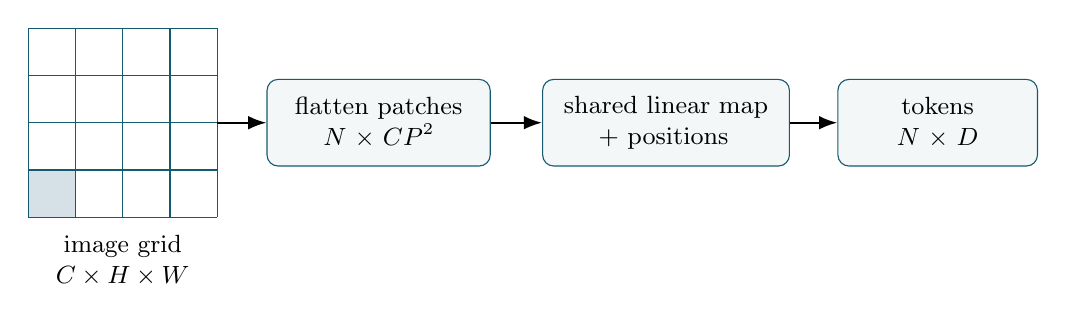
\begin{tikzpicture}[>=Latex,font=\small,
 box/.style={draw=accent,rounded corners,align=center,fill=accent!5,minimum height=11mm}]
\fill[accent!18] (0,0) rectangle (0.6,0.6);
\draw[step=0.6,accent] (0,0) grid (2.4,2.4);
\node[align=center] at (1.2,-0.55) {image grid\\$C\times H\times W$};
\node[box,text width=2.6cm] (flat) at (4.45,1.2) {flatten patches\\$N\times CP^2$};
\node[box,text width=2.9cm] (proj) at (8.1,1.2) {shared linear map\\$+$ positions};
\node[box,text width=2.3cm] (tok) at (11.55,1.2) {tokens\\$N\times D$};
\draw[->,thick] (2.4,1.2) -- (flat);
\draw[->,thick] (flat) -- (proj);
\draw[->,thick] (proj) -- (tok);
\end{tikzpicture}
\caption{Patch embedding for one image. The drawn $4\times4$ grid is
schematic; the example configuration uses $8\times8$ patches.}
\end{figure}

Without positional information, shared token operations and self-attention
are permutation-equivariant: permuting the input tokens permutes the output
tokens in the same way. Mean pooling then makes the classifier invariant to
patch permutations. Learned positions break that unwanted ambiguity.

\textbf{Example sizes.} Resize to $128\times128$, choose $P=16$, $C=3$ and
$D=128$. There are $N=64$ patches, each with $F=768$ pixel values. The input
$(B,3,128,128)$ becomes $(B,64,768)$ and then $(B,64,128)$.
A plain reshape directly from pixels to $(B,N,F)$ is incorrect for the usual
channel-first image layout; spatial axes must first be rearranged.

\newpage
\section{A compact encoder and classification head}
Let $L$ be the number of encoder blocks and $\ell=1,\ldots,L$ the block
index. Layer Normalization (LN), Multi-head Attention (MHA), and a
Feed-Forward Network (FFN) with a Gaussian Error Linear Unit (GELU)
activation form a pre-normalized residual block:
\begin{align}
 U^{(\ell)}&=X^{(\ell-1)}+
   \MHA_\ell\bigl(\LN_{\ell,1}(X^{(\ell-1)})\bigr),\\
 X^{(\ell)}&=U^{(\ell)}+
   \FFN_\ell\bigl(\LN_{\ell,2}(U^{(\ell)})\bigr),\\
 \FFN_\ell(T)&=\operatorname{GELU}(TW_{1,\ell}+b_{1,\ell})
                         W_{2,\ell}+b_{2,\ell}.
\end{align}
$X^{(\ell-1)}$ is the block input, $U^{(\ell)}$ the intermediate result after
attention/residual addition, and $X^{(\ell)}$ the block output; each has shape
$(B,N,D)$. In the FFN, $T$ denotes its input tensor of that shape and $M$ its
hidden feature width. $W_{1,\ell}\in\R^{D\times M}$ and
$W_{2,\ell}\in\R^{M\times D}$ are projection weights; biases
$b_{1,\ell}\in\R^M$ and $b_{2,\ell}\in\R^D$ broadcast over samples and tokens.
Attention mixes tokens; the FFN transforms each token independently.
Residual addition supplies a direct path for information and gradients.

LN operates over the $D$ features of one token. For token row $t\in\R^D$
and feature index $a=1,\ldots,D$,
\begin{equation}
 \LN(t)_a=\gamma_a\frac{t_a-\mu}{\sqrt{\sigma^2+\epsilon}}+\beta_a,
 \quad \mu=\frac1D\sum_{a=1}^{D} t_a,\quad
 \sigma^2=\frac1D\sum_{a=1}^{D}(t_a-\mu)^2.
\end{equation}
$\mu$ is the feature mean, $\sigma^2$ the feature variance, and
$\epsilon=10^{-5}$ a numerical-stability constant. The learned vectors
$\gamma,\beta\in\R^D$ scale and shift each feature. Subscripts $(\ell,1)$,
$(\ell,2)$, and $\mathrm{final}$ identify separately parameterized norms.
After $L$ blocks, normalize, average over tokens, and classify:
\begin{equation}
 g_b=\frac1N\sum_{n=1}^N\LN_{\rm final}(X^{(L)})_{b,n,:},
 \qquad s_b=g_bW_C+b_C^{\mathsf T}\in\R^{365}.
\end{equation}
Here $g_b\in\R^D$ is image $b$'s pooled feature row, $W_C\in\R^{D\times365}$
the classifier weight matrix, $b_C\in\R^{365}$ its bias, and $s_b$ the
365 class logits. The subscript $C$ labels the classifier here. Pooling averages
token index $n=1,\ldots,N$ without adding a classification token.

\begin{center}
\begin{tabularx}{\textwidth}{@{}lY r@{}}
\toprule
Component & Example configuration & Parameters\\\midrule
Patch embedding & $768\to128$, with bias & 98\,432\\
Learned positions & $64\times128$ & 8\,192\\
One attention sublayer & $D=128$, $h=4$, $d=32$, biases & 66\,048\\
One feed-forward sublayer & $128\to512\to128$, biases & 131\,712\\
Two norms per block & Two sets of $\gamma,\beta\in\R^{128}$ & 512\\
Two complete blocks & $L=2$ & 396\,544\\
Final norm & $D=128$ & 256\\
Classifier & $128\to365$, with bias & 47\,085\\\midrule
\textbf{Model total} & Attention/FFN/norm rows above detail each block & \textbf{550\,509}\\
\bottomrule
\end{tabularx}
\end{center}
This is one illustrative baseline, not a claim of optimal accuracy. Choose a
feasible model once, document its parameter count and shapes, and keep it fixed
for all required performance comparisons.

\newpage
\section{A minimal model built from the manual attention module}
This code uses \code{ManualAttention} from Chapter~\ref{ch:attention}.
The model uses linear patch embeddings and mean pooling.
The flattening order matches Equation~\eqref{eq:embedding}.

\begin{lstlisting}[style=python]
class Block(nn.Module):
    def __init__(self, dim, heads, mlp_dim):
        super().__init__()
        self.norm1 = nn.LayerNorm(dim, eps=1e-5)
        self.attn = ManualAttention(dim, heads)
        self.norm2 = nn.LayerNorm(dim, eps=1e-5)
        self.ffn = nn.Sequential(nn.Linear(dim, mlp_dim),
                                 nn.GELU(), nn.Linear(mlp_dim, dim))

    def forward(self, x):
        x = x + self.attn(self.norm1(x))
        return x + self.ffn(self.norm2(x))

class TinyViT(nn.Module):
    def __init__(self, image_size=128, patch=16, dim=128,
                 heads=4, depth=2, mlp_dim=512, classes=365):
        super().__init__()
        if image_size % patch != 0:
            raise ValueError("image_size must be divisible by patch")
        self.image_size, self.patch = image_size, patch
        self.embed = nn.Linear(3 * patch * patch, dim)
        n = (image_size // patch) ** 2
        self.pos = nn.Parameter(torch.zeros(1, n, dim))
        nn.init.normal_(self.pos, std=0.02)
        self.blocks = nn.ModuleList(
            [Block(dim, heads, mlp_dim) for _ in range(depth)])
        self.norm = nn.LayerNorm(dim, eps=1e-5)
        self.head = nn.Linear(dim, classes)

    def forward(self, images):
        B, C, H, W = images.shape
        assert C == 3 and H == W == self.image_size
        p = self.patch
        x = images.reshape(B, C, H // p, p, W // p, p)
        x = x.permute(0, 2, 4, 1, 3, 5)
        x = x.reshape(B, (H // p) * (W // p), C * p * p)
        x = self.embed(x) + self.pos
        for block in self.blocks:
            x = block(x)
        return self.head(self.norm(x).mean(dim=1))

model = TinyViT().to(device=device, dtype=torch.float32)
optimizer = torch.optim.AdamW(model.parameters(), lr=3e-4)
assert sum(p.numel() for p in model.parameters()) == 550509
\end{lstlisting}

In the code, \code{image_size}, \code{patch}, \code{dim}, \code{heads},
and \code{depth} mean $H=W$, $P$, $D$, $h$, and $L$; \code{classes} is the
class count. \code{mlp_dim} is the multilayer perceptron (MLP) hidden width $M$.
Local variables \code{p} and \code{n} are patch side length $P$ and patch
count $N$; \code{x} holds successive representations. The loop visits the
independently learned blocks in \code{ModuleList}.

\newpage
\section{From a smoke test to evidence of learning}
Start on CPU with a tiny batch and check that the model returns $(B,365)$
logits. Check patch ordering with an image containing numbered pixels: each
flattened patch should contain exactly one spatial tile in the chosen channel
order. A shape check alone would not detect a permutation error.

\begin{lstlisting}[style=python]
model.train()
images = torch.randn(2, 3, 128, 128, device=device)
labels = torch.tensor([0, 364], device=device, dtype=torch.long)
optimizer.zero_grad(set_to_none=True)
logits = model(images)
assert logits.shape == (2, 365)
loss = F.cross_entropy(logits, labels)
assert torch.isfinite(loss)
loss.backward()
assert all(p.grad is not None and torch.isfinite(p.grad).all()
           for p in model.parameters())
optimizer.step()
\end{lstlisting}

These assertions are diagnostic and can synchronize the GPU; remove them
from performance measurement windows. Then overfit a few real training images
with deterministic preprocessing. Loss should fall and training accuracy should
rise with enough optimization. If not, check labels, normalization, device
placement, gradient clearing, learning rate, and whether parameters update.
Random labels and random images only check execution, not useful learning.

For 365 nearly uniform class probabilities, cross-entropy is near
$\log(365)\approx5.90$; this is a useful scale check, not a required initial
loss. Uniform random guessing has expected accuracy $1/365\approx0.274\%$.
An overfitted tiny training set can reach high training accuracy while
held-out accuracy remains poor. Report these as different observations.

\section{Relating architecture to performance experiments}
The forward path contains patch rearrangement, projections, normalization,
attention, feed-forward matrix multiplications, pooling, and classification.
Backward propagates through all these operations; the optimizer then reads
and writes parameter state. Attention may not be the largest cost for a small
patch count. Locate the three largest measured CPU self-time operations on
the graph instead of assuming which nodes dominate.

For compilation, first construct an eager reference and a separate candidate
with identical weights. Apply \code{torch.compile(candidate)} to the model,
leaving data loading and logging outside. Compilation may fuse operations or
change dispatch overhead, and an initial call can include compilation work.
Some inputs or control flow cause graph breaks; a new shape may cause
recompilation~\cite{compile}. Warm up forward \emph{and backward} for each
batch size, check output and gradient agreement, and profile the actual
compiled path. Do not infer compiled execution from a TorchLens graph alone.

For the final comparison, train the manual eager, manual compiled, and fastest
supported FP32 SDPA variants from the same initial checkpoint. Keep batch,
data order, optimizer, transformations, and training budget fixed. Save each
run's validation results, throughput windows, and configuration. A faster
implementation is useful only if its computation and learning remain
comparable within documented numerical differences.

\checkpoint{Explain why the classifier produces 365 logits, why positional
parameters depend on $N$, and why changing the patch size would invalidate
a controlled implementation comparison.}

\checkchapterlength
\chapter{Slurm introduction with simple examples}\label{ch:slurm}
\setcounter{chapterstartpage}{\value{page}}
\purpose{Run experiments on allocated compute resources, reproduce the
environment, and retrieve logs, checkpoints, and performance measurements.}

\section{Allocations, tasks, and steps}
Slurm (Simple Linux Utility for Resource Management) schedules work on a shared
cluster. An \emph{allocation} reserves
resources for a job; a \emph{job step} launches processes within it. A
\emph{task} usually means a process, not a CPU thread. One-GPU training here
uses one task with several allocated CPUs for the main process and data
loading. Requesting eight tasks would not automatically make one training
process eight times faster~\cite{slurmquick}.

\begin{tabularx}{\textwidth}{@{}lY@{}}
\toprule
Request & Meaning for a one-node job\\\midrule
\code{--nodes=1} & One compute node.\\
\code{--ntasks=1} & One launched training process.\\
\code{--cpus-per-task=8} & Eight Slurm CPUs for that task; check local core/thread policy.\\
\code{--gres=gpu:rtx3080:1} & A generic resources (GRES) request for one GPU of the named type.\\
\code{--mem=24G} & Host random-access memory (RAM) per node, not GPU device memory.\\
\code{--time=00:10:00} & Ten-minute wall-time limit once running.\\
\code{--partition=p3080} & A site-defined group of eligible nodes.\\
\bottomrule
\end{tabularx}

\code{sbatch} queues a script and returns a job ID; submission does not mean
execution has started. \code{salloc} obtains an allocation for interactive
work, and \code{srun} starts a step (or requests resources when used directly).
Run substantial computation on compute nodes, not the login node.

On Calculon, check the documentation here\footnote{\url{https://fhnw-hpc.pages.fhnw.ch/docs/runjobs/}}.

\section{A short interactive GPU check}
Calculon guide lists \code{p3080} and GPU type \code{rtx3080};
verify live availability and access before use~\cite{calculongpu,calculonpartitions}.
\code{nvidia-smi} is NVIDIA's System Management Interface for inspecting GPUs.
\begin{lstlisting}[style=shell]
sinfo -o "%P %a %l %D %G"
srun --partition=p3080 --nodes=1 --ntasks=1 \
     --gres=gpu:rtx3080:1 --cpus-per-task=8 --mem=24G \
     --time=00:10:00 --pty bash
# Now on the allocated compute node:
source "$VENV_PATH/bin/activate"    # set VENV_PATH beforehand
hostname
nvidia-smi
python -c 'import torch; assert torch.cuda.is_available(); print(torch.cuda.get_device_name(0))'
exit                              # finish the interactive step
\end{lstlisting}
Slurm sets GPU visibility. In a one-GPU job, \code{cuda:0} normally means the
first \emph{visible} GPU, not necessarily physical GPU 0. Preserve
\code{CUDA_VISIBLE_DEVICES}; do not overwrite it to select an unallocated GPU.
Log both the device name and the device of a model parameter and input tensor.
A CUDA-enabled installation alone does not move the computation to the GPU.

\newpage
\section{A batch script for repeatable training}
Save the following example as \code{train.sbatch} when implementing the
challenge. It assumes a prepared virtual environment and a written new training script
\code{train.py} accepting the shown command-line interface (CLI). 
Adjust resource requests to the measured workload.
\code{#SBATCH} directives must precede shell commands, and shell variables
are not expanded inside them~\cite{sbatch}.

\begin{lstlisting}[style=shell]
#!/bin/bash
#SBATCH --job-name=mc2-manual
#SBATCH --partition=p3080
#SBATCH --nodes=1
#SBATCH --ntasks=1
#SBATCH --gres=gpu:rtx3080:1
#SBATCH --cpus-per-task=8
#SBATCH --mem=24G
#SBATCH --time=02:00:00
#SBATCH --output=logs/%x-%j.out
#SBATCH --error=logs/%x-%j.err
set -euo pipefail
cd "$SLURM_SUBMIT_DIR"
: "${VENV_PATH:?Set VENV_PATH before submission}"
: "${PLACES365_ROOT:?Set the prepared shared dataset root}"
: "${RUN_ROOT:?Set your persistent output directory}"
source "$VENV_PATH/bin/activate"
export OMP_NUM_THREADS=2
export MKL_NUM_THREADS=2
export WANDB_MODE=offline
run_dir="${RUN_ROOT}/${SLURM_JOB_ID}"
mkdir -p "$run_dir"
hostname
date -Is
nvidia-smi
python -m pip freeze > "$run_dir/packages.txt"
srun python -u train.py --device cuda:0 --attention manual \
    --batch-size 32 --workers 4 --cpu-threads 2 --epochs 1 \
    --seed 17 --data-root "$PLACES365_ROOT" --output "$run_dir"
\end{lstlisting}

Here \code{PLACES365_ROOT} is the dataset root, \code{RUN_ROOT} the persistent
output root, and \code{run_dir} this job's output directory.
Slurm supplies \code{SLURM_SUBMIT_DIR} (submission directory) and
\code{SLURM_JOB_ID} (job identifier); \texttt{\%x} and \texttt{\%j} expand to the job
name and ID in log paths. Create \code{logs} before submission, since Slurm
opens logs before the script runs. Set and export the three user paths:
\begin{lstlisting}[style=shell]
export VENV_PATH PLACES365_ROOT RUN_ROOT
mkdir -p logs
sbatch train.sbatch
# Example response: Submitted batch job 123456
\end{lstlisting}

\code{OMP_NUM_THREADS} and \code{MKL_NUM_THREADS} bound thread counts for
Open Multi-Processing (OpenMP) and Intel's Math Kernel Library (MKL).
The program must enforce FP32/highest precision and the CLI settings.
CPU threads and loader workers share the allocation: four worker
processes plus two main-process numerical threads are a starting budget, not
a guarantee against oversubscription by third-party libraries. Record actual
thread settings and bound decoding-library threads where needed.

Use a pre-installed environment in batch jobs. Follow the cluster's software
guide\footnote{\url{https://fhnw-hpc.pages.fhnw.ch/docs/software/}} for modules or containers; loading a CUDA toolkit does not install
PyTorch. Keep checkpoints and raw measurements in persistent storage.

\newpage
\section{Monitor, diagnose, and retrieve output}
Use the job ID returned by \code{sbatch}, replacing the illustrative ID below.
\begin{lstlisting}[style=shell]
squeue -u "$USER"                  # queued/running jobs
scontrol show job 123456           # allocation, state, pending reason
tail -f logs/mc2-manual-123456.out  # Ctrl-C stops tail, not the job
sacct -j 123456 --format=JobID,State,Elapsed,ExitCode,AllocCPUS,MaxRSS
scancel 123456                     # only to cancel this job
\end{lstlisting}
\code{sacct} includes job-step records; memory fields may be populated only
for steps and depend on accounting configuration. \code{MaxRSS} is the maximum
resident set size (RSS), a host-memory measure, not peak allocated CUDA
memory~\cite{sacct}. \code{USER} is the shell's username variable. Slurm's
reported completion should also be checked against the program's exit status,
logs, saved metrics, and expected checkpoint.

\begin{tabularx}{\textwidth}{@{}lY@{}}
\toprule
Observation & What to inspect\\\midrule
Pending & Read the scheduler reason: unavailable resources, priority, or limits.\\
CUDA unavailable & Verify a GPU request, visible devices, the Python environment, and CUDA build.\\
CUDA out of memory & Inspect device peak memory and batch size; extra \code{--mem} does not enlarge GPU RAM.\\
Host out of memory & Inspect dataset replication, prefetch queues, worker count, and host RAM request.\\
Time limit & Check elapsed time and checkpoint progress; choose a feasible common training budget.\\
Missing output & Check the submit directory, log parent directory, job state, and stderr.\\
\bottomrule
\end{tabularx}

\section{CPU jobs and storage conditions}
An allocation without GPUs can be can be requested as before; activate the same suitable
environment and run \code{train.py --device cpu} inside it.
\begin{lstlisting}[style=shell]
srun --partition=performance --nodes=1 --ntasks=1 \
     --cpus-per-task=4 --mem=8G --time=00:10:00 --pty bash
# In the allocated shell, activate the environment and run the CPU test.
# Use matching thread counts and record the CPU model; exit when done.
\end{lstlisting}
For CPU-cluster monitoring, pass the matching cluster option to commands such
as \code{squeue -M calc-cpu}. A local laptop CPU versus a cluster GPU comparison
also changes CPU hardware, storage, and software; state those limitations.

For loading experiments, record the actual shared path, cache conditions, and
whether a site-approved node-local scratch directory is used. Copy only the
data needed for the test, respect quotas, and report staging time separately.
Node-local data can disappear at job end; copy results to persistent storage
before releasing the allocation. Repeated reads may be served from RAM, so a
faster second pass does not by itself establish higher drive bandwidth.

Full runs should keep profiling disabled and log at a moderate interval.
Store the job ID with configuration and W\&B metadata. Offline runs can be
synchronized later; retain local metric exports for the notebook regardless
of service availability. Multi-GPU launchers, if attempted as an optional
extension, must avoid multiplying Slurm tasks by launcher-created processes.

\checkchapterlength
\chapter{Computation graphs and profiling}\label{ch:profiling}
\setcounter{chapterstartpage}{\value{page}}
\purpose{Connect model operations to measured time, memory, kernels, and
idle periods without confusing diagnostic traces with representative throughput.}

\section{A graph and a timeline answer different questions}
A computation graph records dependencies: tensors are produced by operations
and consumed by others. A forward visualization describes one executed path
and its shapes. The autograd graph additionally carries backward dependencies;
saved tensors or recomputation make those derivatives possible. Neither is a
literal schedule of CPU instructions or GPU kernels.

\begin{tabularx}{\textwidth}{@{}lY@{}}
\toprule
Tool & Useful evidence and its boundary\\\midrule
Torchview & Forward module/operation structure and tensor shapes; Graphviz renders
the diagram. It is not a device-time profiler~\cite{torchview}.\\
TorchLens & Operation-level relationships, activations, and metadata. Record
version, capture options, and activation retention. Interpret ordinary operation
timings as instrumented host times; identify any supported native-profiler
integration separately~\cite{torchlens}.\\
PyTorch Profiler & Host events, CUDA launches, device activity, shapes, and memory
events. Correlate operations with kernels and the execution timeline~\cite{profiler}.\\
\bottomrule
\end{tabularx}

\begin{lstlisting}[style=python]
import copy
from torchview import draw_graph
graph_model = copy.deepcopy(model).eval()
graph = draw_graph(graph_model, input_data=images, expand_nested=True)
graph.visual_graph.render("forward_graph", format="pdf")
\end{lstlisting}
Choose representative shapes and record that this graph uses evaluation mode.
Capture separately from timing and use the training mode for training traces.
An eager matrix multiplication may dispatch several operations; a compiled or
fused kernel may implement several graph nodes. Views may need no kernel,
whereas making a tensor contiguous can introduce a copy.

\begin{figure}[h]
\centering
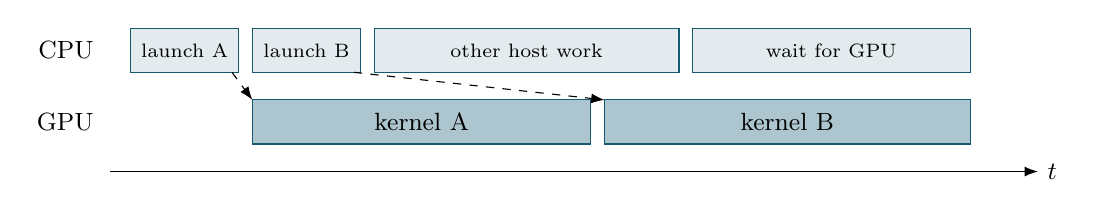
\begin{tikzpicture}[x=0.86cm,y=0.70cm,font=\small,>=Latex]
\node[anchor=east] at (0,2) {CPU};
\node[anchor=east] at (0,0.7) {GPU};
\draw[->] (0.1,-0.2) -- (13.8,-0.2) node[right] {$t$};
\foreach \a/\b/\txt in {0.4/2.0/launch A,2.2/3.8/launch B,4.0/8.5/other host work,8.7/12.8/wait for GPU}
 {\draw[fill=accent!12,draw=accent] (\a,1.6) rectangle (\b,2.4);
  \node at ({(\a+\b)/2},2) {\scriptsize\txt};}
\draw[fill=accent!35,draw=accent] (2.2,0.3) rectangle (7.2,1.1);
\node at (4.7,0.7) {kernel A};
\draw[fill=accent!35,draw=accent] (7.4,0.3) rectangle (12.8,1.1);
\node at (10.1,0.7) {kernel B};
\draw[dashed,->] (1.9,1.6) -- (2.2,1.1);
\draw[dashed,->] (3.7,1.6) -- (7.4,1.1);
\end{tikzpicture}
\caption{Schematic asynchronous execution on one GPU stream; $t$ denotes
elapsed time. Kernel labels A and B identify two operations, not mathematical
variables. Host calls can finish before their kernels; synchronization waits
for queued work.}
\end{figure}

\newpage
\section{Define the measured interval before timing it}
Distinguish three scopes: (i) attention on prepared $Q,K,V$ tensors, with
forward/backward stated explicitly; (ii) a complete training step with inputs
already on the device; and (iii) an end-to-end step including fetching,
transformation, and transfer. State whether attention projections are included.
Never transfer a speedup claim between these scopes without measuring it.

GPU calls usually enqueue work asynchronously~\cite{cudasemantics}. For a
representative wall-clock window, warm up first and synchronize at its
boundaries. Here \code{images} and \code{labels} are already resident; neither
loading nor host logging is measured.
\begin{lstlisting}[style=python]
import time
import statistics

def synchronize(device):
    if device.type == "cuda":
        torch.cuda.synchronize(device)

model.train()
for _ in range(10):  # illustrative; increase until stable
    train_step(model, optimizer, images, labels)
synchronize(device)
times = []
steps = 50
for repeat in range(3):
    synchronize(device)
    start = time.perf_counter()
    for _ in range(steps):
        train_step(model, optimizer, images, labels)
    synchronize(device)
    times.append(time.perf_counter() - start)
latencies = [t / steps for t in times]
rates = [steps * images.shape[0] / t for t in times]
print(statistics.mean(latencies), statistics.stdev(latencies))
print(statistics.mean(rates), statistics.stdev(rates))
\end{lstlisting}

This benchmark updates weights throughout. For implementation comparisons,
restore identical model and optimizer states and use the same input sequence
before each configuration. Warm-up must include optimizer state initialization
and compiled backward work. Measure startup and compilation separately; fixed
warm-up counts alone do not prove steady state.

Let $n$ be the number of measured steps, $B_k$ the image count at step index
$k$, $m=\sum_{k=1}^{n}B_k$ the total image count, and $T$ the window's elapsed
time in seconds. Mean step time is $T/n$ and throughput is $m/T$ images/s. Repeat short
benchmarks at least three times and report a central value, variability,
steps, and images. Window-average step times do not measure individual-step
variability; label the aggregation level. Full training runs need not be
repeated three times, but should report variability across measurement windows.

CUDA events can time an interval on a stream: record a start event, enqueue
work, record an end event, wait for it, then call
\code{start.elapsed_time(end)} (milliseconds). Events may include device idle
gaps between enqueues; they are not a sum of kernel durations. Work on other
streams needs appropriate dependencies. Use wall-clock windows for input-pipeline
throughput, and avoid synchronizing after every operation.

\newpage
\section{Capture short traces and read their timing fields}
Warm up the workload before profiling. The example below captures a short
end-to-end window with a profiler schedule; ensure at least six batches are
available. For resident-input experiments omit fetching and transfer from the
captured loop. Keep the training workload otherwise identical.

\begin{lstlisting}[style=python]
from torch.profiler import profile, ProfilerActivity, record_function
activities = [ProfilerActivity.CPU]
if device.type == "cuda":
    activities.append(ProfilerActivity.CUDA)
model.train()
iterator = iter(train_loader)
with profile(activities=activities, record_shapes=True,
             profile_memory=True, with_stack=False,
             schedule=torch.profiler.schedule(
                 wait=1, warmup=1, active=4, repeat=1)) as prof:
    for _ in range(6):
        with record_function("data_fetch"):
            images, labels = next(iterator)
        with record_function("host_to_device"):
            images = images.to(device, non_blocking=True)
            labels = labels.to(device, non_blocking=True)
        optimizer.zero_grad(set_to_none=True)
        with record_function("forward_and_loss"):
            loss = F.cross_entropy(model(images), labels)
        with record_function("backward"):
            loss.backward()
        with record_function("optimizer"):
            optimizer.step()
        prof.step()
prof.export_chrome_trace("trace.json")
print(prof.key_averages(group_by_input_shape=True).table(
    sort_by="self_cpu_time_total", row_limit=15))
\end{lstlisting}

\begin{tabularx}{\textwidth}{@{}lY@{}}
\toprule
Timing field & Interpretation\\\midrule
CPU self time & Time attributed to a host event excluding its nested child events.\\
CPU inclusive time & Host event duration including nested work; summing parents and
children double-counts that time.\\
GPU/device time & Duration of correlated device activity; it is not the CPU time
spent launching it. Field names can vary by profiler version.\\
Wall time & Elapsed time between measurement boundaries, including waits and
overlap according to the chosen scope.\\
\bottomrule
\end{tabularx}

Open the exported trace in a compatible viewer such as Perfetto. Match
expensive operations to shapes and modules, then inspect kernel launches,
durations, copies, and idle gaps. Include backward and optimizer events.
Aggregate call counts and input shapes, not just operator names. GPU activity
on overlapping streams and nested CPU ranges cannot be added as disjoint wall
time. A host transfer range can end before the corresponding copy completes.

\newpage
\section{Memory and the cost of observing execution}
GPU \emph{allocated} memory is used by live tensors tracked by PyTorch's
allocator. \emph{Reserved} memory includes allocator-managed cached blocks.
Neither is identical to device-wide usage reported by a system monitor;
contexts, libraries, and other processes can contribute to the latter.
Freeing a tensor may reduce allocated memory without reducing reserved memory.

Reset peaks at a documented boundary after warm-up. The following reports
the absolute peak for a window, including its already-live model and input
tensors; it is not just incremental temporary memory~\cite{memoryapi}.
\begin{lstlisting}[style=python]
# CUDA-only, after warm-up; choose the same boundary in every run.
optimizer.zero_grad(set_to_none=True)
torch.cuda.synchronize(device)
torch.cuda.reset_peak_memory_stats(device)
for _ in range(50):
    train_step(model, optimizer, images, labels)
torch.cuda.synchronize(device)
peak_allocated = torch.cuda.max_memory_allocated(device)
peak_reserved = torch.cuda.max_memory_reserved(device)
print(peak_allocated / 2**20, peak_reserved / 2**20)  # MiB
\end{lstlisting}

Parameter count alone underestimates training memory. FP32 parameters and
gradients each require roughly $4P_\theta$ bytes for $P_\theta$ parameters;
two FP32 Adam moment buffers add roughly $8P_\theta$ bytes. Activations,
attention matrices, workspaces, and implementation-specific optimizer
temporaries add further costs. Host-side loader queues consume different memory.
Do not call \code{empty_cache()} between ordinary steps: doing so changes the
allocator workload and is not representative training.

\textbf{Profiler overhead experiment.} Use the same fixed forward workload,
weights, inputs, mode, grad-enabled state, and warm-up for four conditions:
uninstrumented, basic native profiling, profiling with shapes/stacks, and
TorchLens capture. Keep other options constant and record activation-retention
settings. Measure synchronized external wall time; exclude rendering and
file export, and state whether profiler entry/exit and result processing are
included. Record available memory measures for the same boundary.
Let $T_0$ be uninstrumented elapsed time and $T_j$ the time with instrumentation
mode $j$, measured in the same units. The dimensionless slowdown factor is
$\rho_j$; the percentage increase is $\text{overhead}_j$:
\begin{equation}
 \rho_j=T_j/T_0,\qquad
 \text{overhead}_j=100\,(T_j/T_0-1)\%.
\end{equation}
Shape/stack instrumentation and activation retention can add work and extend
tensor lifetimes. Instrumentation can alter dispatch, synchronization, and
memory behavior. Ordinary host operation times from TorchLens cannot establish
a GPU speedup; document the timing source and use supported native device
timings when available. Graph rendering has a different purpose and belongs
outside the measured capture interval.

\textbf{Batch size.} A larger batch can raise step latency but improve images/s
by doing more useful work per launch. Seek a throughput plateau or practical
memory limit using up to four sizes, all with resident inputs. Use traces to
test whether small batches leave launch gaps and whether large batches lengthen
kernels. Sampled GPU utilization reports activity, not achieved floating-point
operations per second (FLOP/s) or memory
bandwidth efficiency; high utilization does not prove efficient execution.

\newpage
\section{Explain pipeline delays, synchronization, and speedups}
For end-to-end experiments, time many steps from fetching inputs through
completed updates. Compare with a matching resident-input reference. Label
\code{next(loader)} waits, transfers, and model work, but remember that loader
workers can prepare future batches while the GPU computes. Under ideal overlap,
steady-state step time approaches the maximum of producer and consumer times;
without overlap it approaches their sum. Real queues and dependencies require
trace evidence.

Hold transformations, shuffle order, storage, pinning, and prefetch policy
fixed while varying worker count. Include zero, small, moderate, and large
counts within the CPU allocation. Pass multiprocessing-only options only when
workers are positive; report total queued batches and separate worker startup
from steady state. Extra workers can contend for CPUs, memory, metadata access,
or storage bandwidth. Waiting for a batch does not identify which of file
access, decoding, transformation, or queueing is responsible.

The main-process profiler does not automatically capture worker internals.
An unchanged model graph under low and high worker counts is expected: file
reads and queues lie outside the model. Compare TorchLens operation metadata
with pipeline traces and throughput, identifying host versus device times.
For storage comparisons, record shared versus local location or first versus
repeated reads and cache conditions; do not infer disk input/output (I/O) solely from
loader waiting time.

\textbf{Accidental synchronization.} \code{loss.item()} must provide a Python
number, so a GPU result must become available on the host. The wait can include
previously queued work. Compare no per-step extraction, extraction every step,
and extraction at a larger interval, holding all model work fixed. Keep console
and network output outside the comparison. Accumulate detached scalar tensors
on device, then extract at logging boundaries; do not retain computation graphs.
Inspect whether host/GPU overlap changes, rather than assuming extraction must
always cause a large slowdown.

\textbf{Limits to component speedups.} In a simplified non-overlapping model,
let $f\in[0,1]$ be attention's fraction of baseline time and $s>0$ its
component speedup (baseline/new attention time). The complete-step speedup
$S$ is baseline/new step time, a dimensionless ratio:
\begin{equation}
 S=\frac{1}{(1-f)+f/s}.
\end{equation}
For $f=0.2$ and $s=4$, $S\approx1.18$. Real overlap can invalidate this
decomposition; use it as a hypothesis and measure the full step. Fusion can
reduce memory traffic and launches, while loading may still dominate training.

For compilation, $\Delta C$ is the additional one-time startup time relative
to eager execution; $t_e$ and $t_c$ are the eager and compiled steady-state
times per step, all in seconds. If $t_c<t_e$, the approximate number of steps
needed to recover that startup cost is $n_{\rm break}$:
\begin{equation}
 n_{\rm break}=\left\lceil\frac{\Delta C}{t_e-t_c}\right\rceil.
\end{equation}
Here $\lceil\cdot\rceil$ rounds up to the nearest integer. This assumes fixed
shapes, no further compilation, and comparable work.
If $t_c\geq t_e$ and $\Delta C>0$, there is no positive amortization benefit.

\checkpoint{For every plot, identify the scope, units, precision, workload,
warm-up, repetitions, timing source, and uncertainty. Use unprofiled throughput
to establish performance, short traces to explain it, and held-out learning
curves to check that the faster execution remains useful.}

\checkchapterlength
\clearpage
\phantomsection
\addcontentsline{toc}{chapter}{References}
\renewcommand{\bibname}{References}
\bibliographystyle{unsrtnat}
\bibliography{ref}
\end{document}
